\documentclass[11pt]{article}

\usepackage[margin=1in]{geometry} 
\usepackage{amsmath,amsthm,amssymb,amsfonts}
\usepackage[czech]{babel}
\usepackage[utf8]{inputenc}
\usepackage{enumitem}
\usepackage{ifthen}
\usepackage{tikz}
\usepackage{tikz-qtree}
\usepackage{caption}
%\usepackage{background}
\usepackage{fancyhdr}
\usepackage{picture}
\usepackage{hyperref}

\pagestyle{fancy}
\fancyhf{}
\rhead{Dominika Regéciová, xregec00}
\lhead{PRL 2016/2017, projekt číslo 3}
\rfoot{\thepage}


\begin{document}
% $$
\section{Mesh multiplication}
Zadáním projektu bylo implementovat pomocí knihovny Open MPI algoritmus Mesh multiplication.\\ 
%dle prezentace do předmětu PRL.\\
Celý program je spouštěn pomocí skriptu: \texttt{./test.sh} a soubory 
\textit{mat1} a \textit{mat2}, obsahující matice. Skript spouští \texttt{mm.cpp}
spolu s \textit{m x k} procesory, kdy mat1 má rozměry \textit{m x n} a mat2 \textit{n x k}.

\section{Rozbor a analýza algoritmu}
Algoritmus běží na \textit{m x k} procesorech, přičemž prvky matic A, B se přivádějí do 
procesorů pomocí 1.\ řádku a 1.\ sloupce procesorového pole. Každý procesor obsahuje proměnnou \textit{c},
reprezentující prvek výsledné matice.\\
V algoritmu s jedním procesorem by se výsledná matice počítala po řádcích a sloupcích,
ve dvou vnořených cyklech, zde jsou pak prováděny paralelně.
Pro výpočet hodnoty \textit{c} procesor čeká, až mu sousední procesory zašlou hodnoty
\textit{a, b}. Hodnotu \textit{a} posílá procesor o sloupec před ním, hodnotu \textit{b} procesor nad ním.
Pokud není hraničním prvek, pošle \textit{a, b} hodnoty svým následujícím sousedům (vedle a pod).
To učiní tolikrát, kolikrát přijme hodnoty \textit{a, b}, což je celkem \textit{n-krát}.\\
Časová složitost $t(n) = m + k - 2$, což odpovídá lineární složitosti.\\
Počet procesorů $p(n) = O(n^2)$. \\
Cena $c(n) = p(n) * t(n) = O(n^3)$.\\
Algoritmus není optimální.

\section{Implementace}
V rámci volání skriptu \texttt{test.sh} probíhá předkontrola vstupu, během kterého jsou načteny řídící číselné hodnoty ze souborů 
-- počet řádků u mat1 a počet sloupců u mat2.\\
Poté se zkontrolují i obracené hodnoty, abych se ujistila, zda je možné matice násobit. Tímto krokem implicitně ověřuji i existenci souborů
a právo z nich číst.\\
Přestože jsem zde, na rozdíl od prvního projektu, neměla vyhrazený procesor pro řízení, procesor s id 0 se i zde
stará o náležitosti k běhu programu navíc.\\
Nejdříve zpracovává vstup a načítá do poměti vstupní matice.
Pokud v této části nastane chyba -- například ve vstupní souboru není dost čísel, či se zde nachází nečíselné hodnoty, pošle
procesor všem svým kolegům zprávu, že program nemůže být dokončen, načež se všichni ukončí.\\
V opačném případě odešle kopii matic prvnímu řádku a prvnímu sloupci procesorů výsledné matice.
Na konci také sesbírá výsledné hodnoty \textit{c}, které dle požadavků vypíše na výstup. \\
Mezitím probíhá algoritmus samotný. Z podstaty problému víme, že počet dvojic hodnot \textit{a, b}, se kterými procesor počítá je shodný s $n$.
Proto jsem místo smyčky, čekající na příchozí hodnoty, implementovala for cyklus. V něm první řada a první sloupec procesorů
postupně čtou hodnoty \textit{a,b} ze svých pamětí a posílají se svým sousedům. Pokud procesor dostane tyto hodnoty, vypočte si aktuální 
\textit{c} a pokud není hraniční v rámci pole, přepošle přijaté hodnoty zase dál.
Trochu speciálně se řeší příjem u procesorů 1.\ řádku a 1.\ sloupce, kdy na některé hodnoty nečekají, protože je mají implicitně přiřazené.

\section{Testování}
Testování jsem spouštěla přes automatizované testy.
Nejdříve jsem testovala správnost implementace algoritmu a porovnávala správnost výsledku.\\
Poté jsem testovala v rozsahu $1$ až $25$ procesorů (včetně), přičemž každý rozsah jsem testovala $10$ krát.
Testy jsem spustila celkově $3$ krát.
Časové hodnoty jsou zprůměrované -- nejdřív průměr $10$ testů a pak průměr $3$ vzniklých hodnot na $n_i$ počet procesorů.\\
Měření jsem prováděla pomocí \textit{MPI\_Wtime()}, kdy jsem měřila od začátku for cyklu, který mi počítá počet odeslaných dvojic hodnot
\textit{a,b}, až do ukončení tohoto cyklu, kdy pak následuje odeslání hodnot procesoru $0$, který výsledek vypíše na výstup.\\
Výsledky odpovídají lineární závislosti, pouze při 4 procesorech jsem trvale získávala podivně vyšší čas, než u zbylých
měřených hodnot.

\begin{figure}[h]
\centering
\includegraphics[scale=0.6]{graf.eps}
\caption{Graf výsledků testování}
\end{figure}

\newpage
\section{Komunikační protokol}
\begin{figure}[h]
\centering
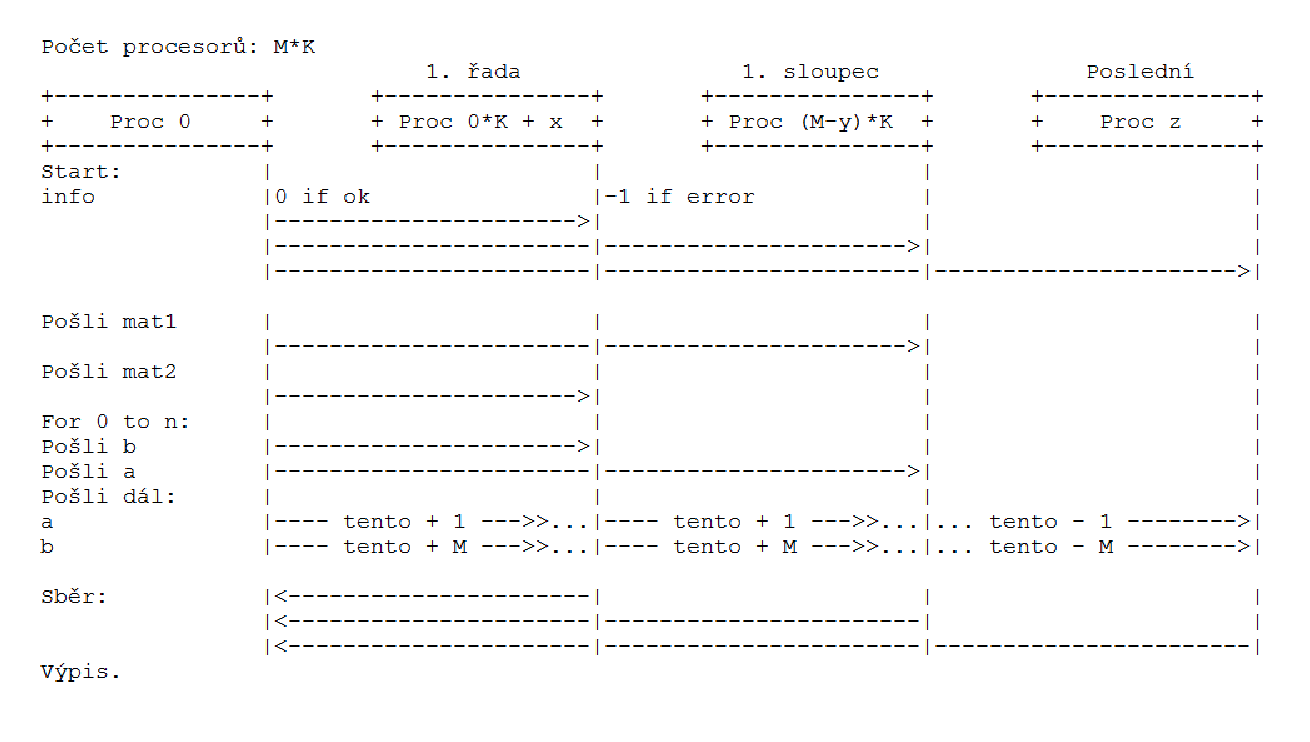
\includegraphics[scale=0.7]{diagram.eps}
\caption{Sekvenční diagram pro n procesorů}
\end{figure}

\section{Závěr}
Znovu jsem pracovala s knihovnou Open MPI pro programování paralelních výpočtů a úspěšně jsem implementovala Mesh multiplication,
včetně kontroly vstupu. Analýza i testování pak ukázaly, že algoritmus pracuje v lineárním čase.
\end{document}
